% You should title the file with a .tex extension (hw1.tex, for example)
\documentclass[a4paper, 11pt]{article}

\usepackage{amsmath}
\usepackage{amssymb}
\usepackage{fancyhdr}
\usepackage{graphicx}

\usepackage[margin=1in]{geometry}

\newcommand{\question}[2] {\vspace{.25in} \hrule\vspace{0.5em}
\noindent{\bf #1: #2} \vspace{0.5em}
\hrule \vspace{.10in}}
\renewcommand{\part}[1] {\vspace{.10in} {\bf (#1)}}

\newcommand{\myname}{Natthakan Euaumpon}
\newcommand{\myemail}{natthakaneuaumpon@gmail.com}
\newcommand{\myhwnum}{4}

\setlength{\parindent}{0pt}
\setlength{\parskip}{5pt plus 1pt}
 
\pagestyle{fancyplain}
\lhead{\fancyplain{}{\textbf{HW\myhwnum}}}      % Note the different brackets!
\rhead{\fancyplain{}{\myname\\ \myemail}}
\chead{\fancyplain{}{ICCS313 }}

\begin{document}

\medskip                        % Skip a "medium" amount of space
                                % (latex determines what medium is)
                                % Also try: \bigskip, \littleskip

\thispagestyle{plain}
\begin{center}                  % Center the following lines
{\Large ICCS313: Assignment \myhwnum} \\
\myname \\
\myemail \\
November 2019 \\
\end{center}
\question{1}{problem1}
Let rod(length,price,cost) be a function to solve for the problem using memoization. Then the recurrence would be:\\
\[
rod(length,price,cost) = 
\begin{cases}
0       & \quad \text{if } smallest\_length > n \geq 0\\
\max\limits_{1\leq i \leq n}(rod(n-l_i)+price[i]-cost)     & \quad \text{if } n >= smallest\_length
\end{cases}
\]
the code is:\\
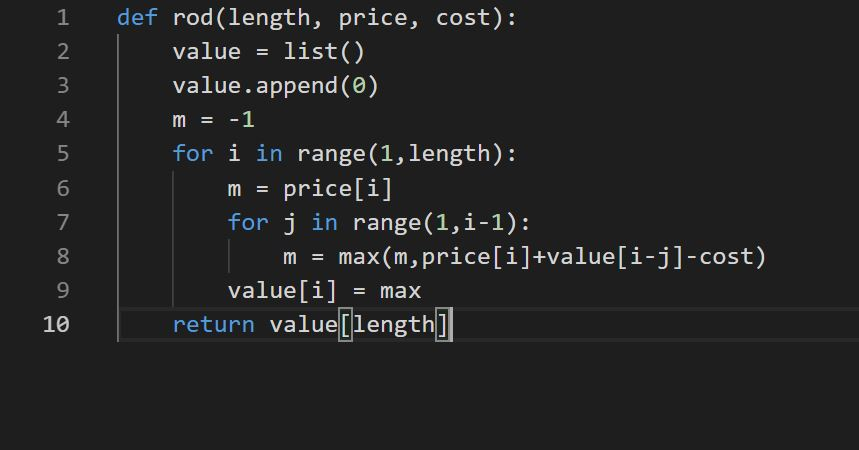
\includegraphics[width=\textwidth]{rod.jpg}\\
Prove that this code give optima solution:\\
Assume for the sake of contradiction that this code does not produce optimal solution. This mean this non-optimal code will produces value a and an optimal code will produce b. Where a < b and a and b are both max value from each code. But the code always give out the maximum possible value. Hence, this code gives out optimal solution.\\
The time complexity for this algorithm is $O(n^{2})$. This is because each loop run O(n) time and it is nested. Other operation only take O(1) time. So the time complexity is $O(n^{2})+O(1) = O(n^{2})$.
\question{2}{Problem2}
Let arr be an array which keep track of the maximum sum and arr[i] is the total sum at position i. So, the total sum of the next position will be arr[i+1]. This mean we can choose the max value between the 2 by comparing. Let say arr[i-1] is k and arr[i] is a. Then the max is either $a+k$ or $a$. So, the recurrence is:\\
\[
arr(i)= 
\begin{cases}
0 & \text{if } i <= 0\\
max(arr(k+a, a)& \text{if } i > 0
\end{cases}
\]
the code is:\\
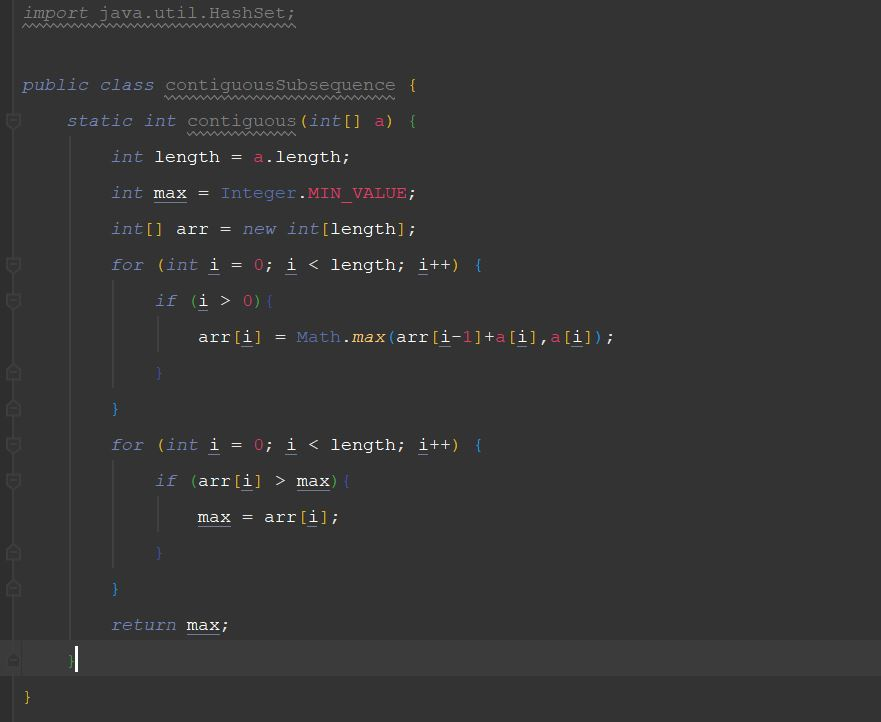
\includegraphics[width=\textwidth]{cs.jpg}\\
This code take in array a as an array if integer which is a given input and return the total sum of the contiguous sub-sequence. Both for-loop take O(n) time each and argument inside both loop take constant time. So, the time complexity for this program is O(n).
\question{3}{Problem3}
Let s be a string input and r be a reverse of s. We can use both string to find the answer. This is because the sting is palindrome. We can find the answer by finding the longest common sub-sequence between s and r. Let length(i,j) be the array which keep track of the maximum length of the common sub-sequence, the recurrence for this code would be:
\[
length(i,j) = 
\begin{cases}
0       & \quad \text{if } i<0 \lor j<0 \\
1+length(i-1,j-1)   & \quad \text{if } s[i] = r[j]\\
max\begin{cases}
length(i-1,j)\\
length(i,j-1)
\end{cases}     & \quad \text{if } s[i] \neq r[j]
\end{cases}
\]
the code is:\\
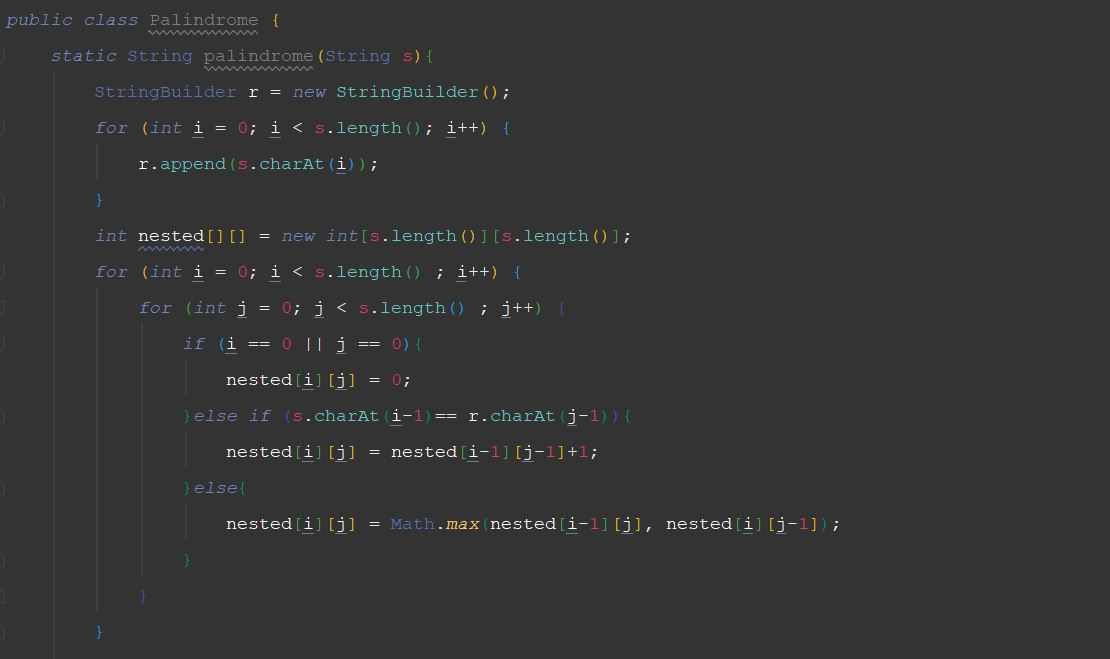
\includegraphics[width=\textwidth]{part1.jpg}\\
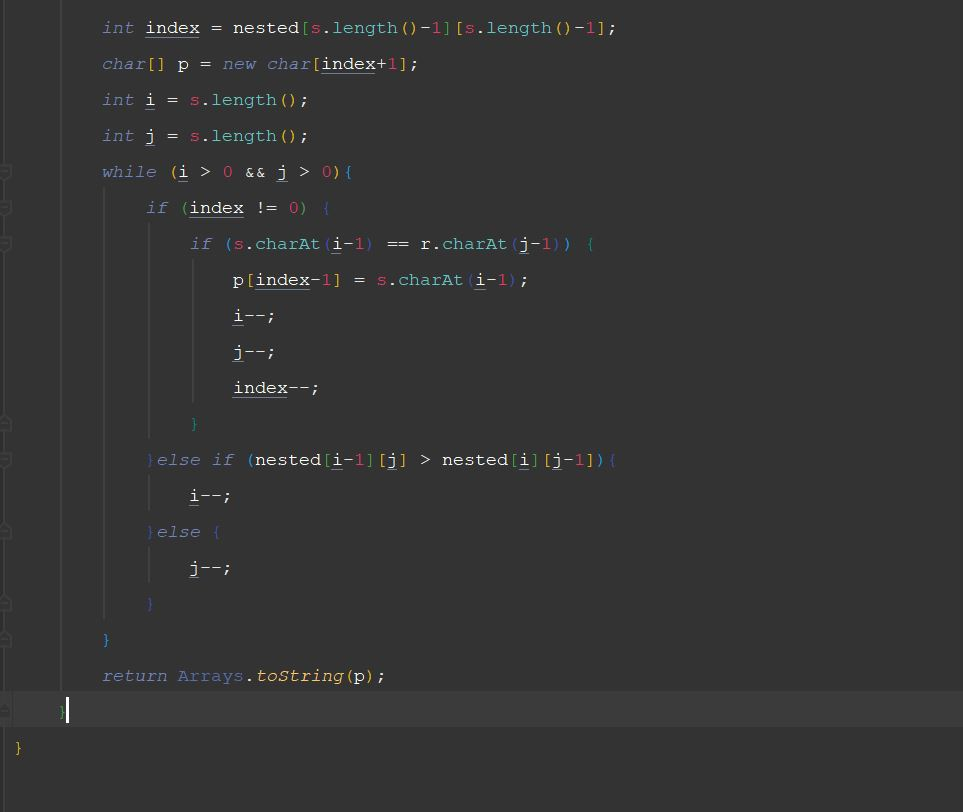
\includegraphics[width=\textwidth]{part2.jpg}\\
The time complexity for this code is $O(n^{2})$. This is because we have one nested for loop which O(n) time each for each loop. We also have one while loop which run within O(n) time complexity. The operation inside and out side the loop all take O(1). So, the time complexity for this program is $O(n^{2})$.
\question{4}{Problem4}
Natthakan Euaumpon\\
@natthakaneuaump1
\end{document}

